% !TeX root = ../dokumentation.tex
\begin{appendix}

\addchap{\langanhang}

{\Large
\begin{enumerate}[label=\Alph*.]
	\item Anhang 1: Funktionsweise Crowdlending
\end{enumerate}
}
\pagebreak
%\includepdf[pages=-,scale=.9,pagecommand={}]{Aufgabenstellung.pdf} % PDF um 10% verkleinert einbinden --> Kopf- und Fußzeile  werden so korrekt dargestellt. Die Option `pages' ermöglicht es, eine bestimmte Sequenz von Seiten (z.B. 2-10 oder `-' für alle Seiten) auszuwählen.

\pagenumbering{roman}
%% Anhang A
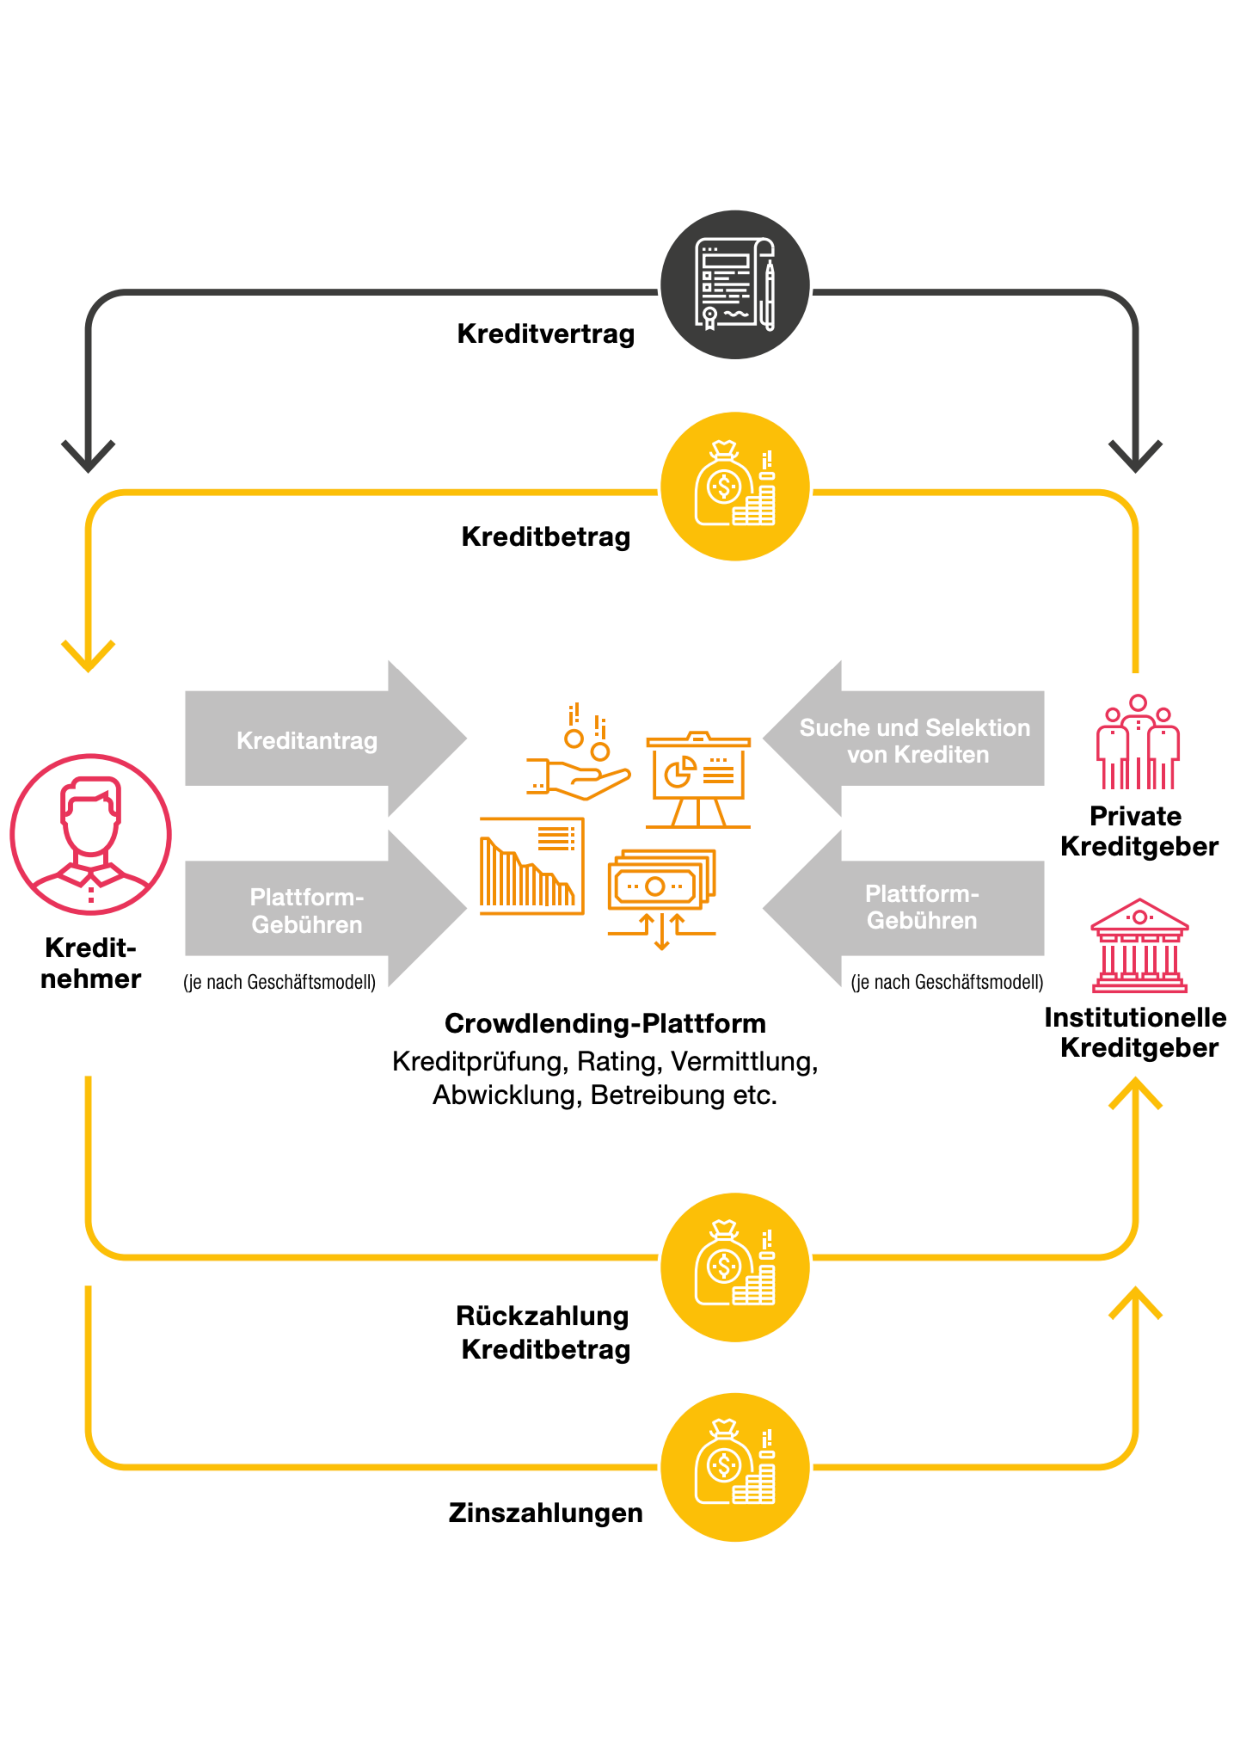
\includepdf[scale=.8,page=1,pagecommand=\section*{A. Funktionsweise Crowdlending\label{sec:A}}]{appendix/Crowdlending.pdf}
\end{appendix}
